% Options for packages loaded elsewhere
\PassOptionsToPackage{unicode}{hyperref}
\PassOptionsToPackage{hyphens}{url}
%
\documentclass[
]{article}
\usepackage{amsmath,amssymb}
\usepackage{iftex}
\ifPDFTeX
  \usepackage[T1]{fontenc}
  \usepackage[utf8]{inputenc}
  \usepackage{textcomp} % provide euro and other symbols
\else % if luatex or xetex
  \usepackage{unicode-math} % this also loads fontspec
  \defaultfontfeatures{Scale=MatchLowercase}
  \defaultfontfeatures[\rmfamily]{Ligatures=TeX,Scale=1}
\fi
\usepackage{lmodern}
\ifPDFTeX\else
  % xetex/luatex font selection
\fi
% Use upquote if available, for straight quotes in verbatim environments
\IfFileExists{upquote.sty}{\usepackage{upquote}}{}
\IfFileExists{microtype.sty}{% use microtype if available
  \usepackage[]{microtype}
  \UseMicrotypeSet[protrusion]{basicmath} % disable protrusion for tt fonts
}{}
\makeatletter
\@ifundefined{KOMAClassName}{% if non-KOMA class
  \IfFileExists{parskip.sty}{%
    \usepackage{parskip}
  }{% else
    \setlength{\parindent}{0pt}
    \setlength{\parskip}{6pt plus 2pt minus 1pt}}
}{% if KOMA class
  \KOMAoptions{parskip=half}}
\makeatother
\usepackage{xcolor}
\usepackage[margin=1in]{geometry}
\usepackage{color}
\usepackage{fancyvrb}
\newcommand{\VerbBar}{|}
\newcommand{\VERB}{\Verb[commandchars=\\\{\}]}
\DefineVerbatimEnvironment{Highlighting}{Verbatim}{commandchars=\\\{\}}
% Add ',fontsize=\small' for more characters per line
\usepackage{framed}
\definecolor{shadecolor}{RGB}{248,248,248}
\newenvironment{Shaded}{\begin{snugshade}}{\end{snugshade}}
\newcommand{\AlertTok}[1]{\textcolor[rgb]{0.94,0.16,0.16}{#1}}
\newcommand{\AnnotationTok}[1]{\textcolor[rgb]{0.56,0.35,0.01}{\textbf{\textit{#1}}}}
\newcommand{\AttributeTok}[1]{\textcolor[rgb]{0.13,0.29,0.53}{#1}}
\newcommand{\BaseNTok}[1]{\textcolor[rgb]{0.00,0.00,0.81}{#1}}
\newcommand{\BuiltInTok}[1]{#1}
\newcommand{\CharTok}[1]{\textcolor[rgb]{0.31,0.60,0.02}{#1}}
\newcommand{\CommentTok}[1]{\textcolor[rgb]{0.56,0.35,0.01}{\textit{#1}}}
\newcommand{\CommentVarTok}[1]{\textcolor[rgb]{0.56,0.35,0.01}{\textbf{\textit{#1}}}}
\newcommand{\ConstantTok}[1]{\textcolor[rgb]{0.56,0.35,0.01}{#1}}
\newcommand{\ControlFlowTok}[1]{\textcolor[rgb]{0.13,0.29,0.53}{\textbf{#1}}}
\newcommand{\DataTypeTok}[1]{\textcolor[rgb]{0.13,0.29,0.53}{#1}}
\newcommand{\DecValTok}[1]{\textcolor[rgb]{0.00,0.00,0.81}{#1}}
\newcommand{\DocumentationTok}[1]{\textcolor[rgb]{0.56,0.35,0.01}{\textbf{\textit{#1}}}}
\newcommand{\ErrorTok}[1]{\textcolor[rgb]{0.64,0.00,0.00}{\textbf{#1}}}
\newcommand{\ExtensionTok}[1]{#1}
\newcommand{\FloatTok}[1]{\textcolor[rgb]{0.00,0.00,0.81}{#1}}
\newcommand{\FunctionTok}[1]{\textcolor[rgb]{0.13,0.29,0.53}{\textbf{#1}}}
\newcommand{\ImportTok}[1]{#1}
\newcommand{\InformationTok}[1]{\textcolor[rgb]{0.56,0.35,0.01}{\textbf{\textit{#1}}}}
\newcommand{\KeywordTok}[1]{\textcolor[rgb]{0.13,0.29,0.53}{\textbf{#1}}}
\newcommand{\NormalTok}[1]{#1}
\newcommand{\OperatorTok}[1]{\textcolor[rgb]{0.81,0.36,0.00}{\textbf{#1}}}
\newcommand{\OtherTok}[1]{\textcolor[rgb]{0.56,0.35,0.01}{#1}}
\newcommand{\PreprocessorTok}[1]{\textcolor[rgb]{0.56,0.35,0.01}{\textit{#1}}}
\newcommand{\RegionMarkerTok}[1]{#1}
\newcommand{\SpecialCharTok}[1]{\textcolor[rgb]{0.81,0.36,0.00}{\textbf{#1}}}
\newcommand{\SpecialStringTok}[1]{\textcolor[rgb]{0.31,0.60,0.02}{#1}}
\newcommand{\StringTok}[1]{\textcolor[rgb]{0.31,0.60,0.02}{#1}}
\newcommand{\VariableTok}[1]{\textcolor[rgb]{0.00,0.00,0.00}{#1}}
\newcommand{\VerbatimStringTok}[1]{\textcolor[rgb]{0.31,0.60,0.02}{#1}}
\newcommand{\WarningTok}[1]{\textcolor[rgb]{0.56,0.35,0.01}{\textbf{\textit{#1}}}}
\usepackage{longtable,booktabs,array}
\usepackage{calc} % for calculating minipage widths
% Correct order of tables after \paragraph or \subparagraph
\usepackage{etoolbox}
\makeatletter
\patchcmd\longtable{\par}{\if@noskipsec\mbox{}\fi\par}{}{}
\makeatother
% Allow footnotes in longtable head/foot
\IfFileExists{footnotehyper.sty}{\usepackage{footnotehyper}}{\usepackage{footnote}}
\makesavenoteenv{longtable}
\usepackage{graphicx}
\makeatletter
\def\maxwidth{\ifdim\Gin@nat@width>\linewidth\linewidth\else\Gin@nat@width\fi}
\def\maxheight{\ifdim\Gin@nat@height>\textheight\textheight\else\Gin@nat@height\fi}
\makeatother
% Scale images if necessary, so that they will not overflow the page
% margins by default, and it is still possible to overwrite the defaults
% using explicit options in \includegraphics[width, height, ...]{}
\setkeys{Gin}{width=\maxwidth,height=\maxheight,keepaspectratio}
% Set default figure placement to htbp
\makeatletter
\def\fps@figure{htbp}
\makeatother
\setlength{\emergencystretch}{3em} % prevent overfull lines
\providecommand{\tightlist}{%
  \setlength{\itemsep}{0pt}\setlength{\parskip}{0pt}}
\setcounter{secnumdepth}{-\maxdimen} % remove section numbering
\usepackage{booktabs}
\usepackage{longtable}
\usepackage{array}
\usepackage{multirow}
\usepackage{wrapfig}
\usepackage{float}
\usepackage{colortbl}
\usepackage{pdflscape}
\usepackage{tabu}
\usepackage{threeparttable}
\usepackage{threeparttablex}
\usepackage[normalem]{ulem}
\usepackage{makecell}
\usepackage{xcolor}
\ifLuaTeX
  \usepackage{selnolig}  % disable illegal ligatures
\fi
\usepackage{bookmark}
\IfFileExists{xurl.sty}{\usepackage{xurl}}{} % add URL line breaks if available
\urlstyle{same}
\hypersetup{
  pdftitle={Untitled},
  pdfauthor={Annika Cleven},
  hidelinks,
  pdfcreator={LaTeX via pandoc}}

\title{Untitled}
\author{Annika Cleven}
\date{2024-11-20}

\begin{document}
\maketitle

\subsection{Project Motivation}\label{project-motivation}

Our project is motivated by ``Epigenetic dysregulation in Alzheimer's
disease peripheral immunity'' (2024, Ramakrishnan). This study
investigates the transcriptional changes in the peripheral immune system
in Alzheimer's disease (AD) using advanced single-cell sequencing
techniques such as scATAC-seq and scRNA-seq. Ramakrishnan and his team
found a considerable amount of open chromatin in the peripheral immune
cells in AD relative to health controls (HC). They also identified
differentially accessible chromatin regions in AD risk genes by checking
the overlap between differentially expressed genes and differentially
accessible regions for AD and HC.

In the investigation, the researchers include a list of the
differentially expressed genes (DEGs) associated with AD, their
associated log 2 fold change, and overlaps between these DEGs and
differentially accessible regions (DARs). While they provide overlaps
between the DARs and DEGs, they do not give any further information. In
our analysis we investigate the distance between DEGs and DARs. A
primary goal of our investigation is to verify the study's binary
overlap results and quantify the distance to and direction from the
nearest gene where the overlap occurs. The researchers have also
annotated, albeit in a very elementary manner, the DEGs' cell type, as
well as the type of the nearest gene. We can also look for trends
between gene and cell type and distance to the nearest gene, which can
further elaborate on the findings of this study.

\subsection{Methods}\label{methods}

The study began by providing information on DARs and DEGs. Using the DEG
names they provided, we annotated the gene coordinates that correspond
with the gene using the \texttt{EnsDb.Hsapiens.v86} library. Using the
two GRanges objects containing the DARs and DEGs, we were interested in
quantifying the overlap DARs and DEGs. We are particularly interested in
the promoter regions of the DEGs and we can extract those from our
GRanges object using the promoters() function. Given that chromatin
should be accessible at promoters for DEGs, whether promoter regions of
DEGs overlap DARs should serve as a positive control.

\begin{Shaded}
\begin{Highlighting}[]
\CommentTok{\# Define promoter regions for DEGs (e.g., 2 kb upstream and 500 bp downstream of the TSS)}
\NormalTok{degs\_promoters }\OtherTok{\textless{}{-}} \FunctionTok{promoters}\NormalTok{(degs\_gr, }\AttributeTok{upstream =} \DecValTok{2000}\NormalTok{, }\AttributeTok{downstream =} \DecValTok{500}\NormalTok{)}
\end{Highlighting}
\end{Shaded}

We also grouped DEGs and DARs by cell type to determine cell-type
specific associations between DEGs and DARs. We calculated distance
between DEG promoters and DARs.

\begin{Shaded}
\begin{Highlighting}[]
\NormalTok{cell\_types }\OtherTok{\textless{}{-}} \FunctionTok{intersect}\NormalTok{(}\FunctionTok{unique}\NormalTok{(degs\_gr}\SpecialCharTok{$}\NormalTok{cell\_type), }\FunctionTok{unique}\NormalTok{(dars\_gr}\SpecialCharTok{$}\NormalTok{cell\_type))}

\CommentTok{\# Step 1: Initialize lists to store results by cell type}
\NormalTok{results\_by\_cell\_type }\OtherTok{\textless{}{-}} \FunctionTok{list}\NormalTok{()}
\NormalTok{dars\_with\_distances\_and\_metadata\_by\_cell\_type }\OtherTok{\textless{}{-}} \FunctionTok{list}\NormalTok{()}

\CommentTok{\# Step 2: Loop over each cell type and compute necessary steps}
\ControlFlowTok{for}\NormalTok{ (ct }\ControlFlowTok{in}\NormalTok{ cell\_types) \{}
  
  \CommentTok{\# Subset DEGs promoters and DARs for the current cell type}
\NormalTok{  degs\_subset }\OtherTok{\textless{}{-}}\NormalTok{ degs\_promoters[degs\_promoters}\SpecialCharTok{$}\NormalTok{cell\_type }\SpecialCharTok{==}\NormalTok{ ct]}
\NormalTok{  dars\_subset }\OtherTok{\textless{}{-}}\NormalTok{ dars\_gr[dars\_gr}\SpecialCharTok{$}\NormalTok{cell\_type }\SpecialCharTok{==}\NormalTok{ ct]}
  
  \CommentTok{\# Check if both subsets are non{-}empty to avoid errors}
  \ControlFlowTok{if}\NormalTok{ (}\FunctionTok{length}\NormalTok{(degs\_subset) }\SpecialCharTok{==} \DecValTok{0} \SpecialCharTok{||} \FunctionTok{length}\NormalTok{(dars\_subset) }\SpecialCharTok{==} \DecValTok{0}\NormalTok{) \{}
    \FunctionTok{warning}\NormalTok{(}\FunctionTok{paste}\NormalTok{(}\StringTok{"Skipping cell type"}\NormalTok{, ct, }\StringTok{"due to empty DEGs or DARs."}\NormalTok{))}
    \ControlFlowTok{next}
\NormalTok{  \}}
  
  \CommentTok{\# Step 3: Calculate the distance to the nearest DEG promoter for each DAR}
\NormalTok{  dist\_to\_nearest }\OtherTok{\textless{}{-}} \FunctionTok{distanceToNearest}\NormalTok{(dars\_subset, degs\_subset)}
  
  \CommentTok{\# Create a vector of distances with NA for unmatched DARs}
\NormalTok{  distances }\OtherTok{\textless{}{-}} \FunctionTok{rep}\NormalTok{(}\ConstantTok{NA}\NormalTok{, }\FunctionTok{length}\NormalTok{(dars\_subset))}
\NormalTok{  distances[}\FunctionTok{queryHits}\NormalTok{(dist\_to\_nearest)] }\OtherTok{\textless{}{-}} \FunctionTok{mcols}\NormalTok{(dist\_to\_nearest)}\SpecialCharTok{$}\NormalTok{distance}
  
  \CommentTok{\# Retrieve indices of matched DARs and DEGs}
\NormalTok{  matched\_dars\_indices }\OtherTok{\textless{}{-}} \FunctionTok{queryHits}\NormalTok{(dist\_to\_nearest)}
\NormalTok{  matched\_degs\_indices }\OtherTok{\textless{}{-}} \FunctionTok{subjectHits}\NormalTok{(dist\_to\_nearest)}
  
  \CommentTok{\# Initialize empty DataFrame for DEG metadata with NA values}
\NormalTok{  n\_dars }\OtherTok{\textless{}{-}} \FunctionTok{length}\NormalTok{(dars\_subset)}
\NormalTok{  deg\_metadata\_full }\OtherTok{\textless{}{-}} \FunctionTok{DataFrame}\NormalTok{(}
    \AttributeTok{seqnames\_deg =} \FunctionTok{rep}\NormalTok{(}\ConstantTok{NA\_character\_}\NormalTok{, n\_dars),}
    \AttributeTok{start\_deg =} \FunctionTok{rep}\NormalTok{(}\ConstantTok{NA\_integer\_}\NormalTok{, n\_dars),}
    \AttributeTok{end\_deg =} \FunctionTok{rep}\NormalTok{(}\ConstantTok{NA\_integer\_}\NormalTok{, n\_dars),}
    \AttributeTok{strand\_deg =} \FunctionTok{rep}\NormalTok{(}\ConstantTok{NA\_character\_}\NormalTok{, n\_dars),}
    \AttributeTok{cell\_type\_deg =} \FunctionTok{rep}\NormalTok{(}\ConstantTok{NA\_character\_}\NormalTok{, n\_dars),}
    \AttributeTok{gene\_name =} \FunctionTok{rep}\NormalTok{(}\ConstantTok{NA\_character\_}\NormalTok{, n\_dars),}
    \AttributeTok{gene\_biotype =} \FunctionTok{rep}\NormalTok{(}\ConstantTok{NA\_character\_}\NormalTok{, n\_dars),}
    \AttributeTok{DAR\_deg\_overlap =} \FunctionTok{rep}\NormalTok{(}\ConstantTok{NA}\NormalTok{, n\_dars),}
    \AttributeTok{log2FC\_deg =} \FunctionTok{rep}\NormalTok{(}\ConstantTok{NA\_real\_}\NormalTok{, n\_dars)}
\NormalTok{  )}
  
  \CommentTok{\# Only proceed if there are any matches}
  \ControlFlowTok{if}\NormalTok{ (}\FunctionTok{length}\NormalTok{(matched\_dars\_indices) }\SpecialCharTok{\textgreater{}} \DecValTok{0}\NormalTok{) \{}
    \CommentTok{\# Extract DEG metadata for matched indices}
\NormalTok{    degs\_seqnames }\OtherTok{\textless{}{-}} \FunctionTok{as.character}\NormalTok{(}\FunctionTok{seqnames}\NormalTok{(degs\_subset))}
\NormalTok{    degs\_start }\OtherTok{\textless{}{-}} \FunctionTok{start}\NormalTok{(degs\_subset)}
\NormalTok{    degs\_end }\OtherTok{\textless{}{-}} \FunctionTok{end}\NormalTok{(degs\_subset)}
\NormalTok{    degs\_strand }\OtherTok{\textless{}{-}} \FunctionTok{as.character}\NormalTok{(}\FunctionTok{strand}\NormalTok{(degs\_subset))}
\NormalTok{    degs\_cell\_type }\OtherTok{\textless{}{-}} \FunctionTok{as.character}\NormalTok{(}\FunctionTok{mcols}\NormalTok{(degs\_subset)}\SpecialCharTok{$}\NormalTok{cell\_type)}
\NormalTok{    degs\_gene\_name }\OtherTok{\textless{}{-}} \FunctionTok{as.character}\NormalTok{(}\FunctionTok{mcols}\NormalTok{(degs\_subset)}\SpecialCharTok{$}\NormalTok{gene\_name)}
\NormalTok{    degs\_gene\_biotype }\OtherTok{\textless{}{-}} \FunctionTok{as.character}\NormalTok{(}\FunctionTok{mcols}\NormalTok{(degs\_subset)}\SpecialCharTok{$}\NormalTok{gene\_biotype)}
\NormalTok{    DAR\_deg\_overlap }\OtherTok{\textless{}{-}} \FunctionTok{as.character}\NormalTok{(}\FunctionTok{mcols}\NormalTok{(degs\_subset)}\SpecialCharTok{$}\NormalTok{DAR\_deg\_overlap)}
\NormalTok{    degs\_log2FC }\OtherTok{\textless{}{-}} \FunctionTok{as.numeric}\NormalTok{(}\FunctionTok{mcols}\NormalTok{(degs\_subset)}\SpecialCharTok{$}\NormalTok{log2FC\_deg)}
    
    \CommentTok{\# Ensure that the lengths of these vectors match the length of degs\_subset}
\NormalTok{    n\_degs }\OtherTok{\textless{}{-}} \FunctionTok{length}\NormalTok{(degs\_subset)}
    
    \CommentTok{\# Now extract the matched metadata}
\NormalTok{    deg\_metadata\_matched }\OtherTok{\textless{}{-}} \FunctionTok{DataFrame}\NormalTok{(}
      \AttributeTok{seqnames\_deg =}\NormalTok{ degs\_seqnames[matched\_degs\_indices],}
      \AttributeTok{start\_deg =}\NormalTok{ degs\_start[matched\_degs\_indices],}
      \AttributeTok{end\_deg =}\NormalTok{ degs\_end[matched\_degs\_indices],}
      \AttributeTok{strand\_deg =}\NormalTok{ degs\_strand[matched\_degs\_indices],}
      \AttributeTok{cell\_type\_deg =}\NormalTok{ degs\_cell\_type[matched\_degs\_indices],}
      \AttributeTok{gene\_name =}\NormalTok{ degs\_gene\_name[matched\_degs\_indices],}
      \AttributeTok{gene\_biotype =}\NormalTok{ degs\_gene\_biotype[matched\_degs\_indices],}
      \AttributeTok{DAR\_deg\_overlap =}\NormalTok{ DAR\_deg\_overlap[matched\_degs\_indices],}
      \AttributeTok{log2FC\_deg =}\NormalTok{ degs\_log2FC[matched\_degs\_indices]}
\NormalTok{    )}
    
    \CommentTok{\# Assign the matched DEG metadata to the corresponding DAR indices}
\NormalTok{    deg\_metadata\_full[matched\_dars\_indices, ] }\OtherTok{\textless{}{-}}\NormalTok{ deg\_metadata\_matched}
\NormalTok{  \}}
  
  \CommentTok{\# Combine DARs, distances, and DEG promoter metadata into a GRanges object}
  \FunctionTok{mcols}\NormalTok{(dars\_subset)}\SpecialCharTok{$}\NormalTok{distance }\OtherTok{\textless{}{-}}\NormalTok{ distances}
  \FunctionTok{mcols}\NormalTok{(dars\_subset) }\OtherTok{\textless{}{-}} \FunctionTok{cbind}\NormalTok{(}\FunctionTok{mcols}\NormalTok{(dars\_subset), deg\_metadata\_full)}
  
  \CommentTok{\# Store the GRanges object by cell type}
\NormalTok{  dars\_with\_distances\_and\_metadata\_by\_cell\_type[[ct]] }\OtherTok{\textless{}{-}}\NormalTok{ dars\_subset}
  
  \CommentTok{\# Optional: Print a summary for debugging}
  \FunctionTok{message}\NormalTok{(}\FunctionTok{paste}\NormalTok{(}\StringTok{"Processed cell type:"}\NormalTok{, ct))}
\NormalTok{\}}

\CommentTok{\# Final: To view the GRanges results by cell type}
\NormalTok{dars\_with\_distances\_and\_metadata\_by\_cell\_type  }\CommentTok{\# GRanges with distances and metadata by cell type}
\CommentTok{\# write\_csv(dars\_with\_distances\_and\_metadata,"working\_data/dars\_with\_distances\_and\_metadata\_by\_cell\_type.csv")}
\end{Highlighting}
\end{Shaded}

Ramakrishnan et al.~identified 217* overlaps, 38 of which were located
within promoter regions of DEGs. We identified 29358 DARs with a
distance of 0 from DEG promoter regions (2 kb upstream and 500 bp
downstream of the TSS). Of our 29358 DARs overlapping DEGs, only 40 were
recorded as overlaps by Ramakrishnan et al., whereas 29318 were not.

Methods: - Describe making GRanges, reasoning for promoter - Why we
separated DARs and DEGs by cell type

Conclusions - Looking at distance stratified by cell type (DAR)

\begin{figure}
\centering
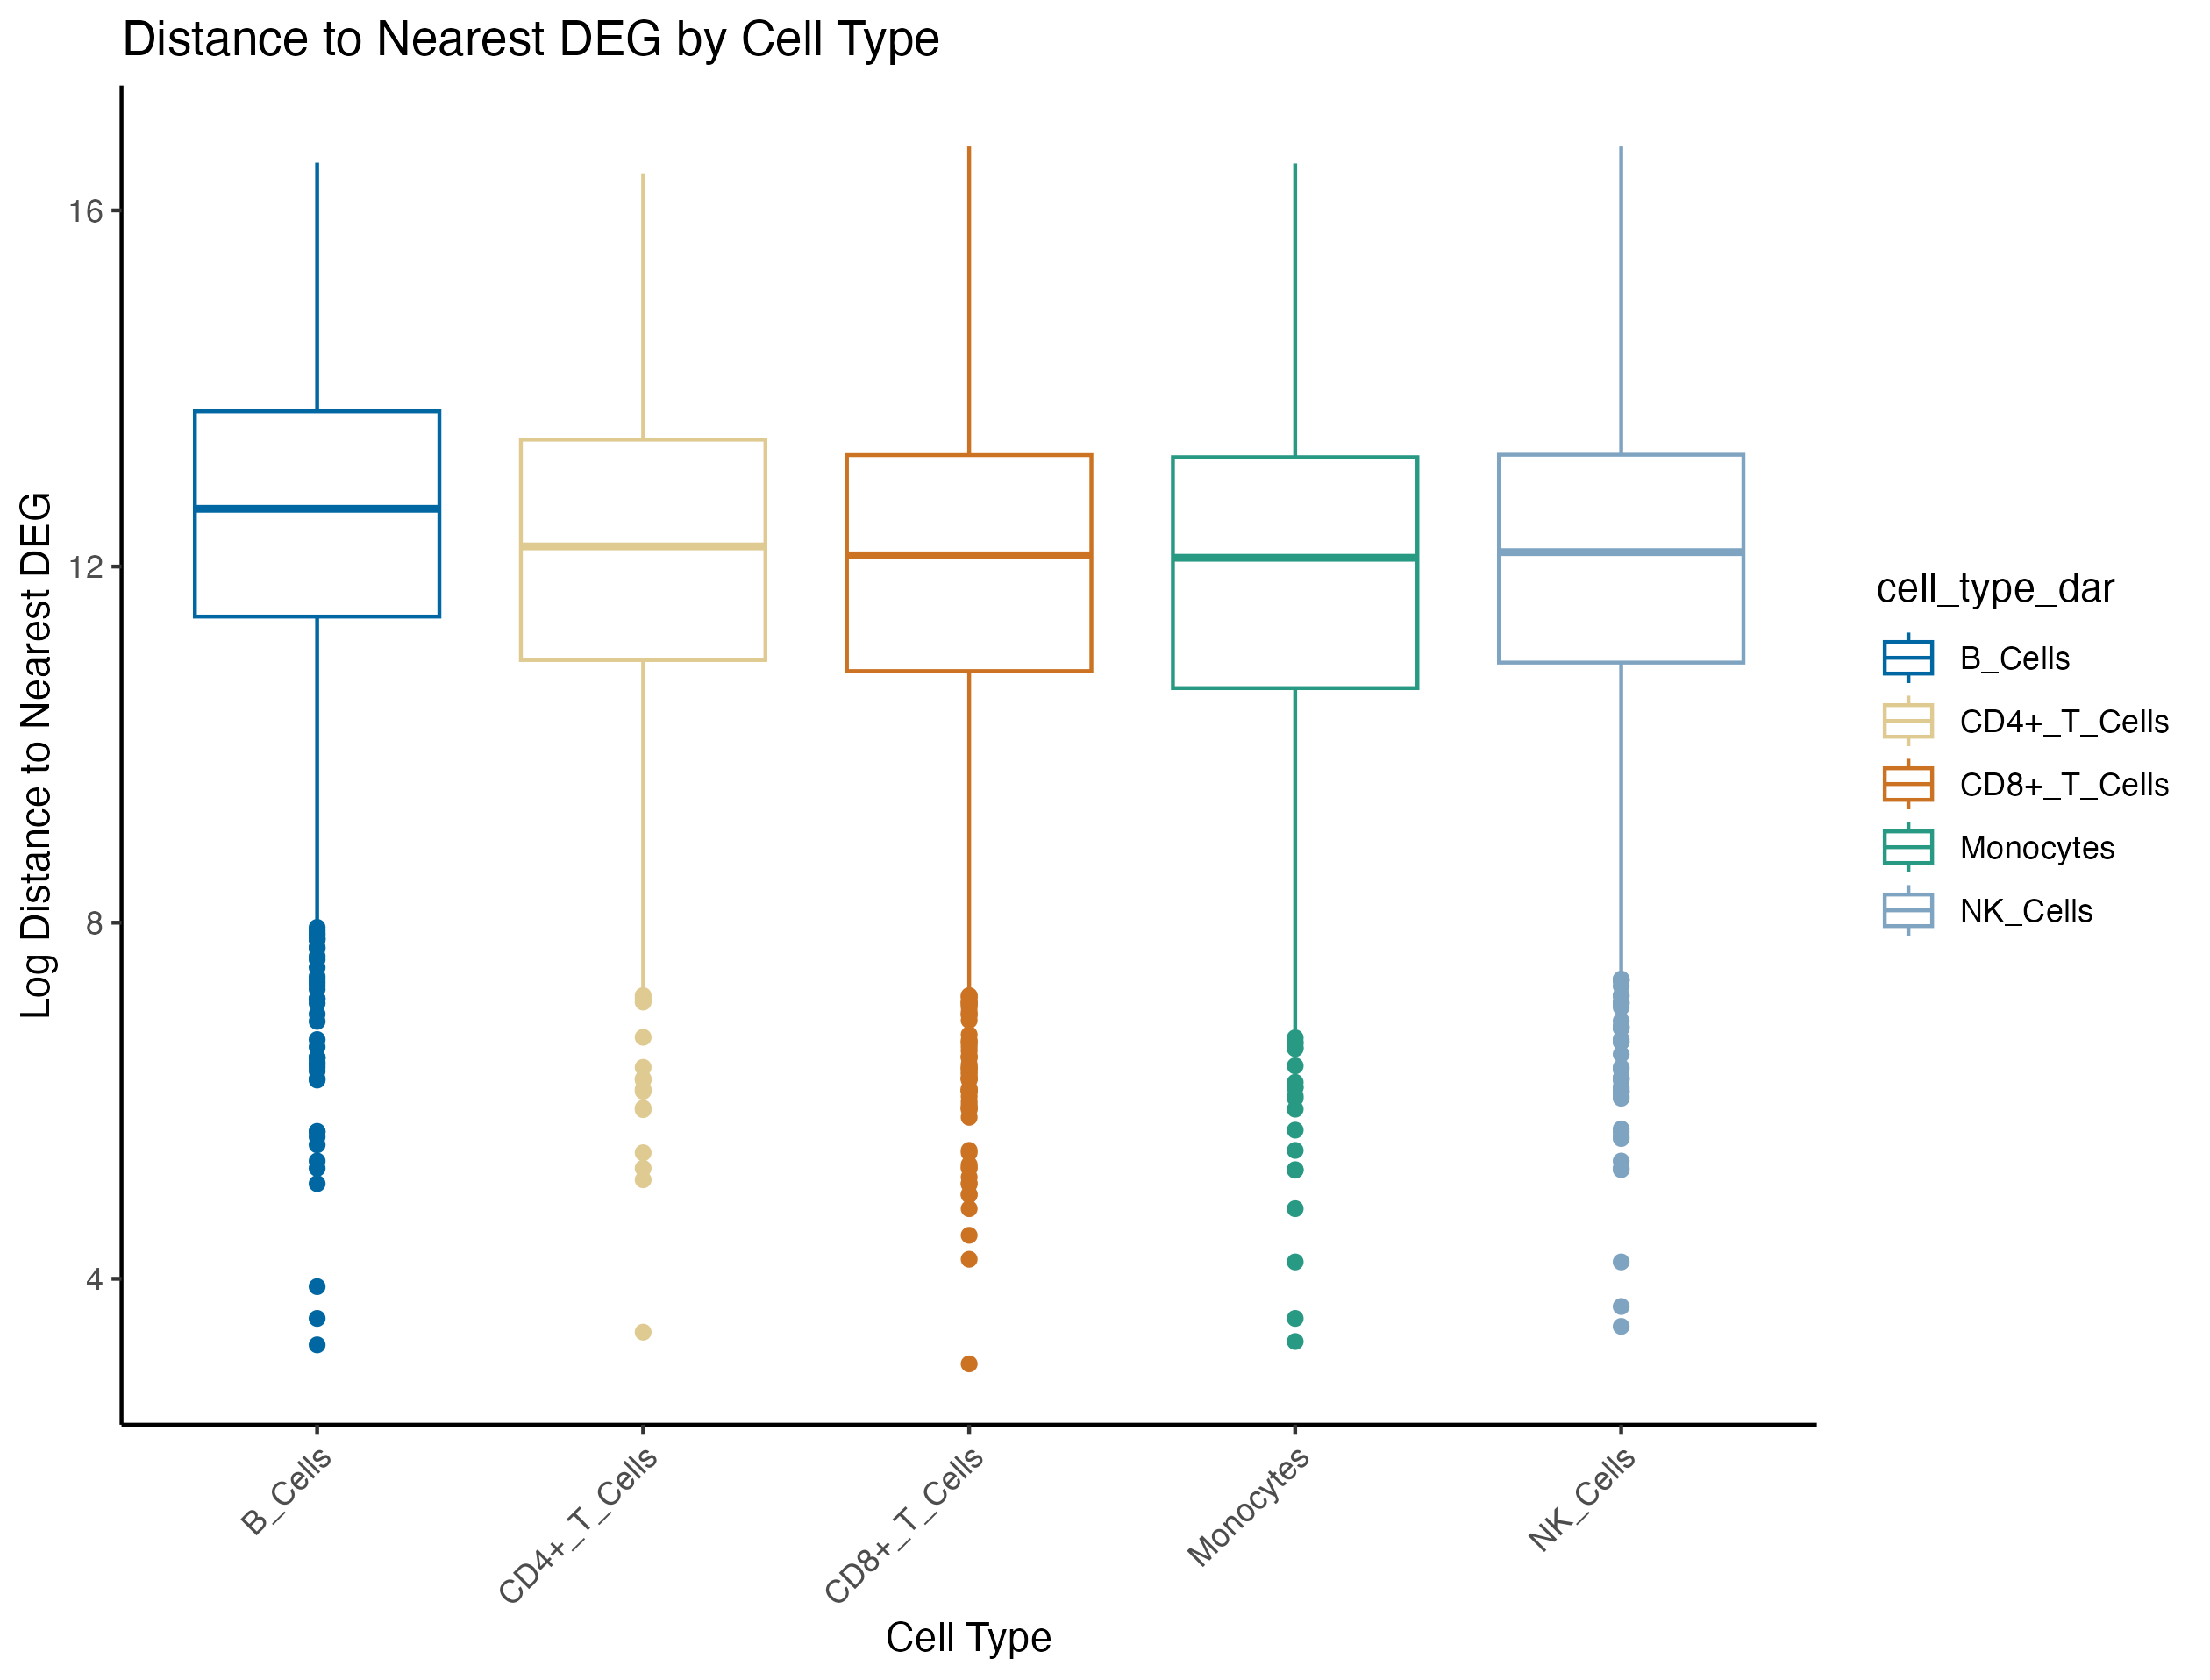
\includegraphics{~/BIOS784-Functional_Genomics/figures/dist_by_celltype_plot.png}
\caption{Distance to Nearest DEG by Cell Type}
\end{figure}

\begin{itemize}
\tightlist
\item
  Look at distance stratified by gene biotype: y - distance, x - biotype
\end{itemize}

\begin{figure}
\centering
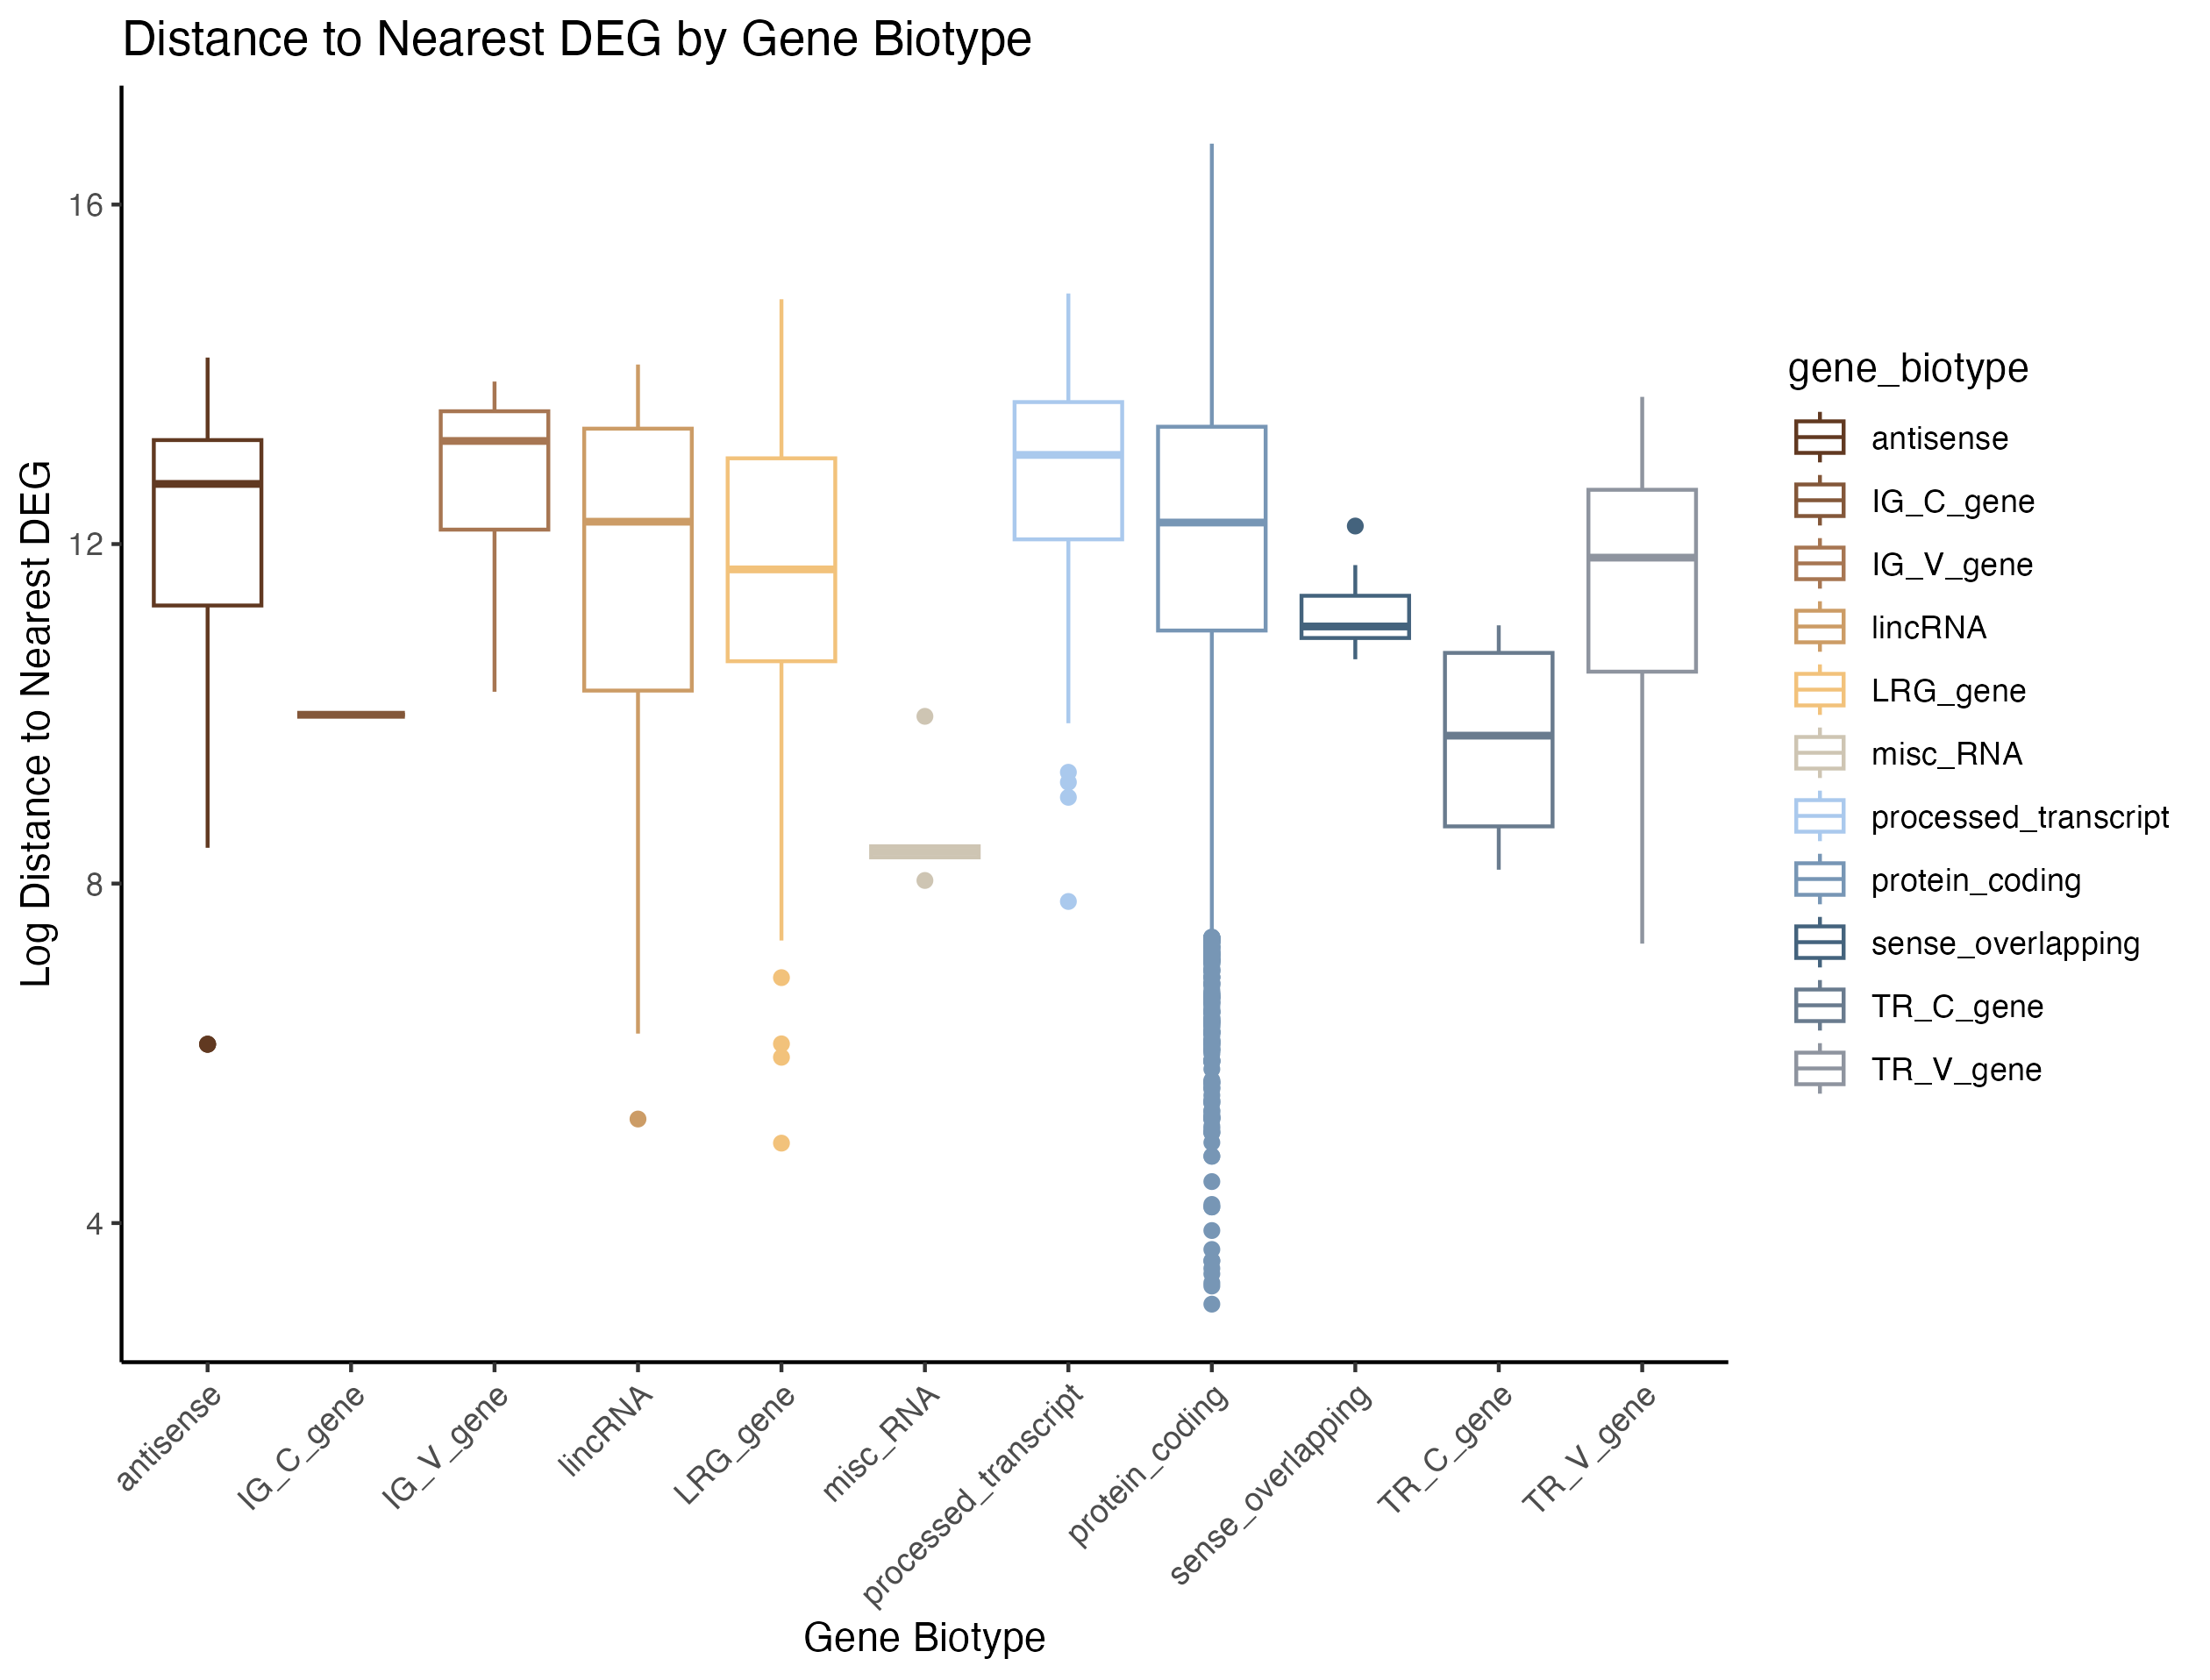
\includegraphics{~/BIOS784-Functional_Genomics/figures/dist_by_biotype_plot.png}
\caption{Distance to Nearest DEG by Cell Type}
\end{figure}

\begin{itemize}
\tightlist
\item
  Distances don't overlap with their DAR/DEG variable. TRUE/FALSE vs
  distances. Results aren't consistent, but they only have a binary
  variable for us to compare results to
\end{itemize}

\begin{longtable}[]{@{}lcl@{}}
\toprule\noalign{}
\ldots\ldots\ldots\ldots. & Overlap & No Overlap \\
\midrule\noalign{}
\endhead
\bottomrule\noalign{}
\endlastfoot
Distance Less than 100 & 8737 & 162 \\
Distance Greater than 100 & 279 & 6 \\
\end{longtable}

\begin{itemize}
\tightlist
\item
  Correlations between logfold changes
\end{itemize}

\end{document}
